%%%%%%%%%%%%%%%%%%%%%%%%%%%%%%%%%%%%%%%%%%%%%%%%%%%%%%%%%%%%%%%%%%%%%%%%%%%%%%%%
% Template for USENIX papers.
%
% History:
%
% - TEMPLATE for Usenix papers, specifically to meet requirements of
%   USENIX '05. originally a template for producing IEEE-format
%   articles using LaTeX. written by Matthew Ward, CS Department,
%   Worcester Polytechnic Institute. adapted by David Beazley for his
%   excellent SWIG paper in Proceedings, Tcl 96. turned into a
%   smartass generic template by De Clarke, with thanks to both the
%   above pioneers. Use at your own risk. Complaints to /dev/null.
%   Make it two column with no page numbering, default is 10 point.
%

% - Munged by Fred Douglis <douglis@research.att.com> 10/97 to
%   separate the .sty file from the LaTeX source template, so that
%   people can more easily include the .sty file into an existing
%   document. Also changed to more closely follow the style guidelines
%   as represented by the Word sample file.
%
% - Note that since 2010, USENIX does not require endnotes. If you
%   want foot of page notes, don't include the endnotes package in the
%   usepackage command, below.
% - This version uses the latex2e styles, not the very ancient 2.09 if
%   stuff.
%
% - Updated July 2018: Text block size changed from 6.5" to 7"
%
% - Updated Dec 2018 for ATC'19:
%
%   * Revised text to pass HotCRP's auto-formatting check, with
%     hotcrp.settings.submission_form.body_font_size=10pt, and
%     hotcrp.settings.submission_form.line_height=12pt
%
%   * Switched from \endnote-s to \footnote-s to match Usenix's policy.
%
%   * \section* => \begin{abstract} ... \end{abstract}
%
%   * Make template self-contained in terms of bibtex entires, to allow
%     this file to be compiled. (And changing refs style to 'plain'.)
%
%   * Make template self-contained in terms of figures, to
%     allow this file to be compiled. 
%
%   * Added packages for hyperref, embedding fonts, and improving
%     appearance.
%   
%   * Removed outdated text.
%
%%%%%%%%%%%%%%%%%%%%%%%%%%%%%%%%%%%%%%%%%%%%%%%%%%%%%%%%%%%%%%%%%%%%%%%%%%%%%%%%
% \documentclass{hotnets22}

% \usepackage{times}  
% \usepackage{hyperref}
% \usepackage{titlesec}

% \hypersetup{pdfstartview=FitH,pdfpagelayout=SinglePage}

% \setlength\paperheight {11in}
% \setlength\paperwidth {8.5in}
% \setlength{\textwidth}{7in}
% \setlength{\textheight}{9.25in}
% \setlength{\oddsidemargin}{-.25in}
% \setlength{\evensidemargin}{-.25in}
% \pagestyle{plain} % removes running headers


% \documentclass[sigplan,10pt,anonymous]{acmart}
\documentclass[letterpaper,twocolumn,10pt]{article}
% \usepackage{usenix}
\usepackage{adjustbox}
\usepackage[english]{babel}
\usepackage{makecell}
\usepackage{usenix}

\usepackage{blindtext}
% \renewcommand\footnotetextcopyrightpermission[1]{} % removes footnote with conference info
% \setcopyright{none}
% \settopmatter{printacmref=false, printccs=false, printfolios=true}


% % Copyright
% \renewcommand\footnotetextcopyrightpermission[1]{} % removes footnote with conference info
% % Copyright
% \renewcommand\footnotetextcopyrightpermission[1]{} % removes footnote with conference info
% \setcopyright{none}
% \settopmatter{printacmref=false, printccs=false, printfolios=true}
% % DOI
% \acmDOI{}
% % ISBN
% \acmISBN{}
% %Conference
% \acmConference[Submitted for review to SIGCOMM NAIC Workshop]{}
% \acmYear{2024}
% %\copyrightyear{}
% %% {} with no args suppresses printing of the price
% \acmPrice{}

% to be able to draw some self-contained figs
\usepackage{tikz}
\usepackage{amsmath}

% inlined bib file
\usepackage{filecontents}

% \pagenumbering{roman}
%\usepackage{times}
%\usepackage{natbib}

\usepackage{tikz}
\usepackage{xcolor}
\usepackage{xspace}
\usepackage{tikz}
\usepackage{pifont}
\usepackage[english]{babel}
\usepackage{blindtext}
\usepackage{lipsum}
%\usepackage{subfigure}

\usepackage[ruled,vlined,linesnumbered]{algorithm2e}
\usepackage{booktabs}

\usepackage{filecontents}
\usepackage{xspace}
% \usepackage{subfig}
\usepackage{xcolor}
\usepackage{hhline}
\usepackage{multirow}
\usepackage{soul}
\newtheorem{definition}{Definition}
\usepackage{array}
\usepackage{comment}
\usepackage{listings}
\usepackage{amssymb}
\usepackage{dsfont}
\usepackage{algorithmic}
\usepackage{xurl}
\usepackage{setspace}
\usepackage[flushleft]{threeparttable}
\urlstyle{rm}
\usepackage{enumitem}
\usepackage{enumerate}
\usepackage{float}
\usepackage{subcaption}
\usepackage{graphicx}
\usepackage{breqn}



% for table in appendix
\usepackage{caption}
\usepackage{ltablex}
% \usepackage{stfloats}

\usepackage{ifluatex}

\usepackage{outlines}
% \usepackage{hyperref}
\newtheorem{insight}{Insight}

%\usepackage{titlesec}
%\titleformat{\subsubsection}[runin]{\normalfont\normalsize\bfseries}%{\thesubsubsection}{1em}{}
\captionsetup[figure]{belowskip=0pt}
\captionsetup[figure]{skip=0pt}
\captionsetup[table]{belowskip=0pt}
\captionsetup[table]{skip=0pt}
\setlist[enumerate]{noitemsep, topsep=0pt}
\setlist[itemize]{noitemsep, topsep=0pt}

%\usepackage{titlesec}

\usepackage[compact]{titlesec}
\renewcommand{\paragraph}[1]{\noindent\textbf{#1}}
\titlespacing{\paragraph}{0pt}{*0.5}{*1}
\setlength{\textfloatsep}{5pt plus 0pt minus 2.0pt}
\titlespacing\section{0pt}{*1.8}{*1.1}
\titlespacing\subsection{0pt}{*1.5}{*1.1}
\titlespacing\subsection{0pt}{*1.3}{*0.8}
\usepackage{booktabs}

\begin{document}

\newcommand*{\affmark}[1][*]{\textsuperscript{#1}}
\newcommand*{\affaddr}[1]{#1}

%\title{CAIP: Context Aware Iterative Prompting for LLM-Powered Router Misconfiguration Detection

\title{CAIP: Detecting Router Misconfigurations with Context-Aware Iterative Prompting of LLMs}
\author{Paper \#722, \pageref{endOfBody} pages body, \pageref{LastPage} pages total}
% \renewcommand{\shortauthors}{X. Jiang, et al}
\newcommand{\eg}{{\it e.g.}}
\newcommand{\ie}{{\it i.e.}}
\newcommand{\etal}{{\it et al.}}
\newcommand{\sysname}{{CAIP}}
%!TEX root = main.tex
%!TEX spellcheck = en_US
\newcommand{\edit}[1]{{\color{black} #1}}
% \newcommand{\cc}[1]{{\color{cyan!70!blue}{(Wan: #1)}}}
\newcommand{\jc}[1]{{\footnotesize\color{orange}{(JC: #1)}}}
\newcommand{\jcedit}[1]{{\color{orange} #1}} 
\newcommand{\chase}[1]{{\color{brown}{(Chase: #1)}}}
\newcommand{\todo}[1]{{\color{red}{(TODO: #1)}}}
\definecolor{darkkhaki}{rgb}{0.74, 0.72, 0.42}
\newcommand{\sr}[1]{{\color{cyan!70!blue}{(Siddhant: #1)}}}
\newcommand{\jack}[1]{{\color{purple}{(Jack: #1)}}}
\newcommand{\aaron}[1]{{\color{teal}{(Aaron: #1)}}}



% \newcommand{\shan}[1]{}
% \newcommand{\hank}[1]{ }
% \newcommand{\mm}[1]{ }
% \newcommand{\cc}[1]{ }
% \newcommand{\jc}[1]{ }
% \newcommand{\yh}[1]{ }
% \newcommand{\kt}[1]{ }

% \newcommand{\todo}[1]{{\color{red}{#1}}}

\newcommand{\smallindent}{\hphantom{N}}



% \newcommand{\shan}[1]{}
% \newcommand{\hh}[1]{}
% \newcommand{\hank}[1]{}
% \newcommand{\mm}[1]{} 
% \newcommand{\cc}[1]{}
%  \newcommand{\jc}[1]{}
% \newcommand{\yh}[1]{}

% \newcommand{\name}{\textsc{METIS}\xspace}
% \newcommand{\name}{\textsc{Name}\xspace}

\newcommand{\vspacesize}{0.2cm}


\newcommand{\fillme}{{\bf XXX}\xspace}

\newcommand*\circled[1]{\tikz[baseline=(char.base)]{
            \node[shape=circle,fill,inner sep=2pt] (char) {\textcolor{white}{\footnotesize{#1}}};}}

\newcommand{\name}{NAME\xspace}




\newcounter{packednmbr}
\newenvironment{packedenumerate}{\begin{list}{\thepackednmbr.}{\usecounter{packednmbr}\setlength{\itemsep}{0.5pt}\addtolength{\labelwidth}{-4pt}\setlength{\leftmargin}{2ex}\setlength{\listparindent}{\parindent}\setlength{\parsep}{1pt}\setlength{\topsep}{0pt}}}{\end{list}}
\newenvironment{packeditemize}{\begin{list}{$\bullet$}{\setlength{\itemsep}{0.5pt}\addtolength{\labelwidth}{-4pt}\setlength{\leftmargin}{2ex}\setlength{\listparindent}{\parindent}\setlength{\parsep}{1pt}\setlength{\topsep}{2pt}}}{\end{list}}
\newenvironment{packedpackeditemize}{\begin{list}{$\bullet$}{\setlength{\itemsep}{0.5pt}\addtolength{\labelwidth}{-4pt}\setlength{\leftmargin}{\labelwidth}\setlength{\listparindent}{\parindent}\setlength{\parsep}{1pt}\setlength{\topsep}{0pt}}}{\end{list}}
\newenvironment{packedtrivlist}{\begin{list}{\setlength{\itemsep}{0.2pt}\addtolength{\labelwidth}{-4pt}\setlength{\leftmargin}{\labelwidth}\setlength{\listparindent}{\parindent}\setlength{\parsep}{1pt}\setlength{\topsep}{0pt}}}{\end{list}}
\let\enumerate\packedenumerate
\let\endenumerate\endpackedenumerate
\let\itemize\packeditemize
\let\enditemize\endpackeditemize


\newcommand{\tightcaption}[1]{\vspace{-0.15cm}\caption{{\normalfont{\textit{{#1}}}}}\vspace{-0.3cm}}
\newcommand{\tightsection}[1]{\vspace{-0.3cm}\section{#1}\vspace{-0.2cm}}
\newcommand{\tightsectionstar}[1]{\vspace{-0.17cm}\section*{#1}\vspace{-0.08cm}}
\newcommand{\tightsubsection}[1]{\vspace{-0.25cm}\subsection{#1}\vspace{-0.1cm}}
\newcommand{\tightsubsubsection}[1]{\vspace{-0.01in}\subsubsection{#1}\vspace{-0.01cm}}


\newcommand{\bigO}{\mathrm{O}}
\newcommand{\twlog}{w.l.o.g.\xspac}

\newcommand{\myparashort}[1]{\vspace{0.05cm}\noindent{\bf {#1}}~}
\newcommand{\mypara}[1]{\vspace{0.05cm}\noindent{\bf {#1}:}~}
\newcommand{\myparatight}[1]{\vspace{0.02cm}\noindent{\bf {#1}:}~}
\newcommand{\myparaq}[1]{\smallskip\noindent{\bf {#1}?}~}
\newcommand{\myparaittight}[1]{\smallskip\noindent{\emph {#1}:}~}
\newcommand{\question}[1]{\smallskip\noindent{\emph{Q:~#1}}\smallskip}
\newcommand{\myparaqtight}[1]{\smallskip\noindent{\bf {#1}}~}

\newcommand{\cmark}{\ding{51}}%
\newcommand{\xmark}{\ding{55}}%


% \definecolor{codegreen}{rgb}{0,0.6,0}
% \definecolor{codegray}{rgb}{0.5,0.5,0.5}
% \definecolor{codepurple}{rgb}{0.58,0,0.82}
% \definecolor{backcolour}{rgb}{0.95,0.95,0.92}

% \lstdefinestyle{overleaf_style}{
%     backgroundcolor=\color{backcolour},   
%     commentstyle=\color{codegreen},
%     keywordstyle=\color{magenta},
%     numberstyle=\tiny\color{codegray},
%     stringstyle=\color{codepurple},
%     basicstyle=\ttfamily\footnotesize,
%     breakatwhitespace=false,         
%     breaklines=true,                 
%     captionpos=b,                    
%     keepspaces=true,                 
%     numbers=left,                    
%     numbersep=5pt,                  
%     showspaces=false,                
%     showstringspaces=false,
%     showtabs=false,                  
%     tabsize=2
% }

\definecolor{backcolour}{rgb}{0.96,0.96,0.96}
\definecolor{codegray}{rgb}{0.5,0.5,0.5}
\definecolor{deepblue}{rgb}{0,0,0.6}
\definecolor{deepred}{rgb}{0.6,0,0}
\definecolor{deepgreen}{rgb}{0,0.5,0}
\lstdefinestyle{mystyle}{
    backgroundcolor=\color{backcolour},   
    commentstyle=\color{codegreen},
    morekeywords={self, True},
    keywordstyle=\color{deepblue},
    numberstyle=\tiny\color{codegray},
    emph={MyClass,__init__,EncodingType,Image},
    emphstyle=\color{deepred},
    stringstyle=\color{deepgreen},
    basicstyle=\ttfamily\footnotesize,
    breakatwhitespace=false,         
    breaklines=true,                 
    captionpos=b,                    
    keepspaces=true,                 
    numbers=left,                    
    numbersep=5pt,                  
    showspaces=false,                
    showstringspaces=false,
    showtabs=false,                  
    tabsize=1
}

\maketitle

%!TEX root = main.tex
%!TEX spellcheck = en_US

\begin{abstract}

%Misconfiguration detection in router configurations is crucial for maintaining network stability, security, and performance.
%Traditional methods like formal model checkers and consistency checkers either rely on manual rule definitions, requiring heavy domain expertise, or assume deviations from standard settings always indicate errors, overlooking context-specific configurations. 
%LLM-based Q\&A models have emerged as a solution by leveraging transformer-based architectures pre-trained on vast datasets, including networking documents. These models enhance misconfiguration detection by capturing both syntax and semantic relationships, benefiting from pre-learned context on how configurations should function.
%However, detecting misconfigurations often requires task-specific context from the actual configuration files for accurate inference. Current methods such as partition-based prompting fail to capture this, missing crucial context and interdependencies spread across the files, resulting in incomplete or inaccurate detection.

% LLM-based Q&A models have emerged as a solution by leveraging transformer architectures and pre-training on vast datasets including networking-related documents, making them adept at capturing common syntax and semantic misconfigruation from general understand of network configruation context. 
% The limitations have led to the adoption of LLM-based Q\&A models, which leverage transformer-based architectures to process and interpret both the syntax and semantics of configurations. Transformers, with their self-attention mechanisms, excel at capturing long-range dependencies and contextual relationships within sequences of text by pre-training on vast datasets, including networking-related documents.
% Yet, the prevalent use of partition-based prompting in LLMs—where configuration files are divided into isolated sections for analysis—fails to account for the interdependencies and contextual relationships that are spread across the configuration file, leading to incomplete or inaccurate misconfiguration detection.

Model checkers and consistency checkers detect critical errors in router
    configurations, but these tools require significant manual effort to
    develop and maintain. 
    % LLM-based Q\&A models have emerged as a promising
    % alternative, because transformer-based models pre-trained on vast datasets
    % include context for interpreting router configurations.
    LLM-based Q\&A models have emerged as a promising 
    alternative, allowing users to query partitions of configurations 
    through prompts and receive answers based on learned 
    patterns, thanks to transformer models pre-trained on 
    vast datasets that provide generic configuration context for interpreting 
    router configurations.
    % Yet, detecting
    % misconfigurations often requires network-specific context from the actual
    % configurations to enable accurate inference.
    Yet, current method of partition-based prompting often
    do not provide enough network-specific context 
    from the actual
    configurations to enable accurate inference.
    We introduce a Context-Aware Iterative Prompting (\sysname{}) framework that
    automates network-specific context extraction and optimizes LLM prompts
    for more precise router misconfiguration detection. \sysname{} addresses
    three challenges: (1) efficiently mining relevant context from complex configuration files, (2) accurately distinguishing between
    pre-defined and user-defined parameter values to prevent irrelevant
    context from being introduced, and (3) managing prompt context overload with
    iterative, guided interactions with the model.
    % Our evaluations using
    % synthetic and real-world configurations show that \sysname{} significantly
    % improves the accuracy of LLM-based misconfiguration detection,
    % outperforming or matching existing methods across all tested scenarios.
 Our evaluations on synthetic and real-world configurations show that 
 \sysname{} improves misconfiguration detection accuracy by more than 
 30\% compared to partition-based LLM approaches, model checkers, and 
 consistency checkers, uncovering over 20 previously undetected 
 misconfigurations in real-world configurations.

\end{abstract}

\pagestyle{plain}

%-------------------------------------------------------------------------------
\begin{sloppypar}
%!TEX root = main.tex
%!TEX spellcheck = en_US

\section{Introduction}
\label{sec:intro}

Misconfiguration detection in router configurations is crucial for maintaining the stability, security, and performance of network infrastructures. Whether due to overlooked errors in existing setups or mistakes introduced during configuration changes, misconfigurations can lead to black holes, unintended access routes, or inefficient routing paths. %These disruptions not only compromise the network’s integrity but also result in costly downtimes or security breaches. 
For instance, a misconfigured access control list (ACL) may allow unauthorized traffic, exposing the network to potential attacks, while a poorly defined routing policy may create loops, making services inaccessible and degrading performance.

Researchers and practitioners have developed a plethora of tools for detecting network misconfigurations. Model checkers~\cite{fogel2015general, beckett2017general, abhashkumar2020tiramisu, prabhu2020plankton, zhang2022sre, steffen2020netdice, ye2020hoyan, ritchey2000using,al2011configchecker, jeffrey2009model} model a network's routing and forwarding behaviors based on protocol semantics and device configurations, and check whether engineer-specified reachability and resilience policies are satisfied. Consistency checkers~\cite{kakarla2024diffy, kakarla2020finding, le2006minerals, feamster2005detecting, tang2021campion,le2008detecting,le2006characterization} compare configurations within and across devices and flag inconsistencies and deviations from best practices. LLM-based Q\&A tools~\cite{bogdanov2024leveraging,chen2024automatic,wang2024identifying,liu2024large, wang2024netconfeval, lian2023configuration} parse configuration files and query pre-trained sequential transformer models for detecting both syntactical and subtle semantic issues.

A fundamental feature of all configurations checkers is their reliance on {\em context}. Model checkers require protocol specifications, current (or proposed) device configurations, and forwarding policies; consistency checkers require configurations from multiple devices and a set of best practices; and LLMs rely on incorporating a sufficient number of relevant configuration lines in query prompts. Moreover, the correctness and completeness of this context impacts configuration checkers' accuracy. For example, providing an incomplete set of forwarding policies, best practices, or too few lines of configurations in LLM prompts may cause misconfigurations to be missed. Similarly, improperly modeling protocol semantics~\cite{birkner2021metha, ye2020hoyan}, excluding certain configurations~\cite{xu2023netcov}, or supplying unrelated configuration lines in LLM prompts~\cite{liskavets2024prompt,tian2024examining,khurana2024and, shvartzshnaider2024llm} may cause false alarms.

While some context is easy to provide---\eg, current config\-urations---many forms of context require significant manual effort. For example, a detailed understanding of routing protocols, their interactions~\cite{le2007rr}, and vendor-specific nuances~\cite{ye2020hoyan} is required to accurately model networks' routing and forwarding behaviors. Similarly, awareness of packet and route filter semantics is required to accurately detect inconsistencies in filter configurations~\cite{kakarla2020finding}.
%As another example, forwarding policies are rarely recorded and only certain types of policies can be reverse-engineered from configurations~\cite{birkner2020config2spec, kheradmand2020anime}. 

Since LLMs are trained on vast volumes of data---which likely includes protocol standards, vendor documentation, and sample configurations---a significant amount of context is already embedded in large-scale pre-trained models (PTMs)~\cite{qiu2020pre}. However, such pre-learned context often need to be supplemented with task-specific context, which details the specific configurations and states within the current configuration file under analysis. Including this task-specific context in the prompt is essential for detecting misconfigurations unique to the file or device.
Current approaches like feeding the entire file into a single prompt can result in context and token overload, diluting the model's focus. Conversely, partitioning the file into multiple prompts disrupts interdependencies between configuration lines, causing incomplete context and potential errors to be missed. Therefore, task-specific context must be carefully extracted and structured to ensure proper focus and coverage.

In this paper, we introduce a new framework, Context-Aware Iterative Prompting (\sysname{}), designed to automate context extraction and optimize prompting to LLMs for accurate router misconfiguration detection. We identify three key challenges in realizing this framework and provide solutions to address them:

\mypara{Challenge 1 - Efficient and Accurate Context Mining}
Network configuration files are often lengthy and complex, with interrelated lines that require careful context extraction. The challenge lies in efficiently identifying and extracting relevant context to reduce computational costs and avoid introducing irrelevant information that could impair the accuracy of misconfiguration detection. \textbf{Solution}: We address this by leveraging the hierarchical structure of configuration files, modeling them as trees where each line is a unique path from root to parameter value. This allows us to systematically mine three types of context—neighboring, similar, and referenceable configurations—ensuring that the LLM receives the most relevant information for accurate analysis.

\mypara{Challenge 2 - Parameter Values Ambiguity in Referenceable Context}
Configurations contain both pre-defined and user-defined parameter values, with the latter requiring context for proper interpretation. When extracting referenceable context, misidentifying these can lead to irrelevant context mining and increased computational overhead. \textbf{Solution}: To accurately differentiate these values, we implement an existence-based method within the configuration tree, identifying user-defined values by their presence as intermediate nodes in other paths. Additionally, we use a majority-voting approach to resolve ambiguities, ensuring consistency in how values are treated across different contexts.

\mypara{Challenge 3 - Managing Context Overload in Prompts}
Even with precise context extraction, the volume of relevant information can be extensive, risking prompt overload when fed into LLMs. Excessive context can dilute relevance, reduce coherence, and degrade the model’s performance, necessitating strategies to manage and streamline the input effectively. \textbf{Solution}: Our framework mitigates this by allowing the LLM to iteratively request specific types of context, refining the prompt based on the model’s feedback. This approach prevents overload and enhances the model’s ability to focus on the most relevant information, leading to more precise misconfiguration detection.

We evaluate our framework through two distinct case studies: (1) synthetic change verification: using configuration snapshots from real networks, we introduce synthetic modifications to simulate potential changes that network operators may make (both correct and incorrect). We demonstrate that the model accurately infers and detects these changes. (2) comprehensive real configuration snapshot verification: we exhaustively run \sysname{} on configuration snapshots from a medium-sized campus network to detect overlooked misconfigurations in real-world environments. Our evaluation shows that \sysname{} consistently outperforms or matches the accuracy of existing methods across all scenarios.
\section{Background and Motivation}
\label{sec_background}
Network misconfigurations are a common and persistent issue, often leading to significant security vulnerabilities, performance degradation, or even network outages. Given the complexity and interdependency of modern network configurations, manually identifying and rectifying these errors has become impractical, driving the need for automated solutions.

Existing methods for misconfiguration detection in networks fall primarily into two categories: model checking methods and data-mining approaches. Model checkers, such as \textit{Batfish}~\cite{fogel2015general} and \textit{Minesweeper}~\cite{beckett2017general}, analyze the structure and behavior of network configurations by either deriving a logical model of the network or emulating the data-plane that would emerge from the current configuration.
For example, Batfish detects network configuration errors by analyzing both control and data planes before configurations are applied, checking for routing loops, syntax errors, and configuration inconsistencies. While model checkers are popular, they rely heavily on predefined rules and require domain expertise to set up. Moreover, they often struggle with the nuanced, interconnected nature of configuration files, where the meaning and impact of a single line can depend heavily on its broader context.
On the other hand, Minesweeper verifies properties like reachability and load-balancing by converting network configurations into logical formulas.
In contrast to model-checking approaches, data-mining tools such as \textit{Diffy}~\cite{kakarla2024diffy} and \textit{Minerals}~\cite{le2006minerals} take a statistical approach by learning common configuration patterns and detecting deviations as potential errors.
For instance, Diffy learns configuration templates and identifies anomalies by comparing new configurations to learned patterns while Minerals applies association rule mining to detect misconfigurations by learning local policies from router configuration files. However, data-mining approaches tend to oversimplify configurations by treating deviations from standard patterns as misconfigurations, leading to false positives when valid configurations deviate for context-specific reasons.


Given the shortcoming of these existing tools,
people have increasingly turned to Large Language Models (LLMs) for misconfiguration detection~\cite{bogdanov2024leveraging,chen2024automatic,wang2024identifying,liu2024large, wang2024netconfeval} due to their advanced ability to understand and process complex contextual information embedded within network configurations. A state-of-the-art tool in this category is Ciri~\cite{lian2023configuration}, a LLM-based configuration validation framework.

LLMs, specifically transformer-based models~\cite{vaswani2017attention,hill2024transformers,lin2022survey}, excel at capturing intricate relationships between configuration elements by leveraging self-attention mechanisms that dynamically weigh the importance of each token (or configuration parameter) in relation to others, regardless of their distance within the file. This allows LLMs to attend to both local and global dependencies, enabling them to recognize not only syntax and pattern anomalies but also to infer potential misconfigurations based on the underlying semantics of the configuration. The use of position encodings ensures that the order of elements in a configuration file is considered, allowing LLMs to assess the correctness of parameters based on their sequence. Additionally, most LLMs rely on the use of large-scale pre-trained models (PTMs) trained on vast amounts of data~\cite{qiu2020pre}, particularly generative pretrained tranformers (GPTs)~\cite{achiam2023gpt,touvron2023llama,shanahan2024talking,taylor2023galactica,brown2020language,chowdhery2023palm}, enabling them to generalize effectively across various tasks.
These distinct advantages have spurred the use of LLMs across diverse domains~\cite{carion2020end,sheng2019nrtr,neil2020transformers,parmar2018image,chen2021developing,gulati2020conformer}, making their application in network misconfiguration detection a natural progression.

Through this architecture, LLMs are able to generalize across different contexts, even for unseen configurations, enabling them to detect subtle errors that might arise from interactions between different configuration elements—issues often missed by conventional tools. As networks become more complex, with increasingly interdependent components, LLMs' ability to holistically analyze configurations and understand the intent behind them makes them a powerful tool for enhancing the accuracy and reliability of misconfiguration detection.


Despite the powerful capabilities of LLMs, their application in misconfiguration detection still faces a critical challenge: how to effectively prompt these models to ensure they can make accurate detection decisions. Specifically, when examining a particular line in a network configuration file, it’s essential to extract all relevant context—other configuration lines that are related and can potentially aid in misconfiguration detection. Without proper context, the LLM’s ability to detect issues is diminished~\cite{liskavets2024prompt,tian2024examining,khurana2024and, shvartzshnaider2024llm}.

The naive approach would be to feed the entire configuration file to the LLM, either all at once or progressively, and let the model handle the detection. This method, while straightforward, is highly inefficient due to the inherent token length limitations of LLMs~\cite{xue2024repeat,yu2024breaking,gu2023mamba}. More critically, flooding the model with all the configuration data can lead to context overload~\cite{lican,li2024long,qian2024long}, a known issue where the presence of excessive and irrelevant information dilutes the LLM’s capacity to focus on what’s important. This not only reduces the model’s performance but can also result in missing key misconfigurations or generating false positives due to irrelevant context. Network configuration files can be large and complex, with numerous unrelated sections, making it impractical to handle all lines equally without careful context management.

A common solution to this problem has been partition-based prompting, where the configuration file is broken down into smaller chunks or sections, typically based on the order in which the configuration appears in the file. These chunks are then individually fed to the LLM for misconfiguration detection. This approach reduces the token load per prompt and ensures that the model is not overwhelmed by a massive context. However, this method introduces a new set of problems: by treating sections in isolation, it often fails to account for interdependent lines that reside in different parts of the file. Network configurations, unlike typical documents, often contain parameters that interact with or depend on other sections that may not be adjacent in the file.

For example, consider a configuration file where one chunk defines firewall rules and another chunk, further down the file, defines routing policies. A misconfiguration in the firewall rules might depend on how the routing policies are set up, but because partition-based prompting processes these sections independently, this critical context is lost. This is particularly detrimental for detecting dependency-related misconfigurations, where proper detection requires understanding how different sections of the configuration work together. If the partitioned chunk only contains locally adjacent lines that define completely different things, then critical context from other parts of the configuration will be missing, and the model will fail to make accurate inferences.
Another example is where a routing policy is defined in one section of the file and referenced by several other rules throughout the configuration. Partitioning might place the definition and its references into separate chunks, leading the LLM to miss vital connections between them, or worse, misinterpret their relationships.

In this paper, we develop a tool that addresses these specific challenges by introducing a context-aware, iterative prompting mechanism. This mechanism is designed to carefully manage and extract relevant context for each configuration line under review, ensuring that the LLM is provided with sufficient information without overloading it. The following sections detail the challenges we encountered and explain the methodologies we developed to solve them.
\section{Method}
\label{sec:method}

\begin{figure*}[t]
    \centering
    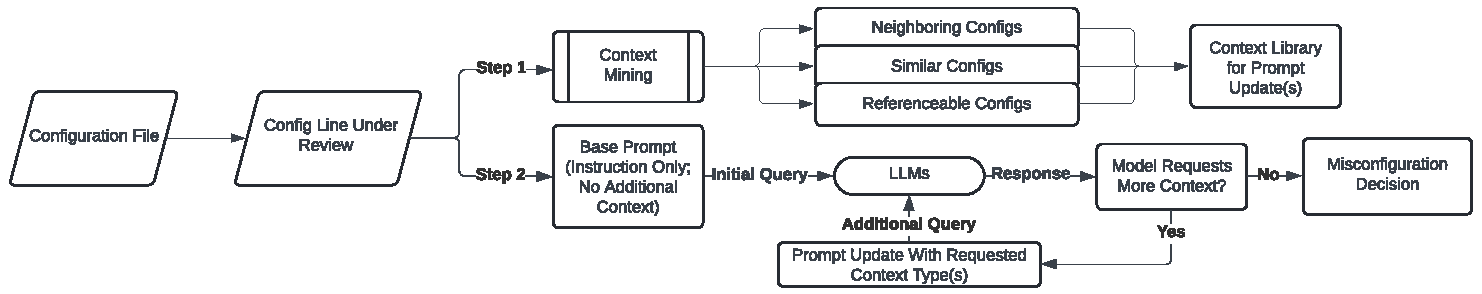
\includegraphics[width=\linewidth]{figs/caip_space.pdf}
    \caption{\sysname{} system overview.}
    \label{fig:overview}
\end{figure*}

To address the limitations of partition-based prompting, we design Context-Aware Iterative Prompting (\sysname{}), which consists of two components as shown in Figure~\ref{fig:overview}: an context mining component and an iterative prompting component. These components work together to automate the process of context extraction and prompt interaction with LLMs, enabling more accurate router misconfiguration detection.


\mypara{1. Context Mining Component}
In this phase, \sysname{} automatically mines all relevant context for a given configuration line under examination. Relevance here refers to configurations that, while not necessarily directly related, provide important insights—such as neighboring configurations, similar lines applied in different contexts, or referenceable configurations that define key parameters.

% This context mining is designed to be both efficient and precise, extracting only the most relevant data from the configuration file without flooding the system with unnecessary information.

\mypara{2. Iterative Prompting Component}
Once the relevant context has been mined, the online component engages the LLM through an iterative prompting process. Instead of overwhelming the model with all the extracted context at once, \sysname{} interacts with the LLM in a guided, sequential manner.



We detail the challenges encountered in designing these two components and present the solutions.
% that enable \sysname{} to perform effective context extraction and interactive prompting for misconfiguration detection.

\subsection{Context Mining}\label{mining_method}
\subsubsection{Challenge 1 - Efficient and accurate context mining}
\label{challenge_1}
Configuration files are often lengthy and complex, consisting of multiple interrelated lines that define various aspects of a system's behavior. When analyzing a specific configuration line, it is crucial to efficiently identify and extract the relevant context to reduce the computational burden on LLMs and minimize the risk of introducing irrelevant information that could degrade the accuracy of misconfiguration detection. This task is challenging because, while these configurations are typically written in a machine and human-readable format, automating the process of context extraction requires a deep understanding of the hierarchical and interconnected nature of the configuration data. For example, in a network configuration, a line that specifies an access control rule might be dependent on prior lines that define network segments or user roles. Without properly extracting and including this context in prompt, the LLM might misinterpret the rule, leading to false positives or missed misconfigurations.

To address this challenge, we leverage two observations:

\mypara{1. Hierarchical Structure of Configuration Files}
    Configuration files are typically written in a structured, hierarchical format that can be effectively modeled as a tree, as shown in the example in Figure~\ref{fig:tree}. In this tree representation (\(T\)), each node (\(V\)) corresponds to a specific configuration element, and edges represent the relationships or dependencies between these elements. Let any unique path \(
P = \{ V_1 \rightarrow V_2(P) \rightarrow V_3(P) \rightarrow \dots \rightarrow V_k(P) = v_k(P) \}
\) in this tree have \(k\) nodes, where the value of \(k\) can vary depend on the path taken. The root node (\(V_1\)) represents the entry point of the configuration file (thus, it functions solely as the root of the tree, providing no semantic meaning, and remains identical regardless of the path taken), while the immediate following node (\(V_2(P)\)) corresponds to the broadest configuration category in this specific path. Intermediate nodes at subsequent levels (\( V_2(P), V_3(P), \dots, V_{k-1}(P) \)) represent increasingly nested configuration sections or subcategories, each refining the configuration context. The leaf node \(V_k(P)\) (or parameter node) represents the final configurable parameter in this path, with the associated value \(v_k(P)\), \ie, parameter values, indicating the specific configuration setting. A unique configuration line is thus a complete path in the tree, starting from the root node and terminating at a parameter node, where the path reflects the hierarchical structure and relationships defined in the configuration file.
\begin{figure}[t]
    \centering
    \fbox{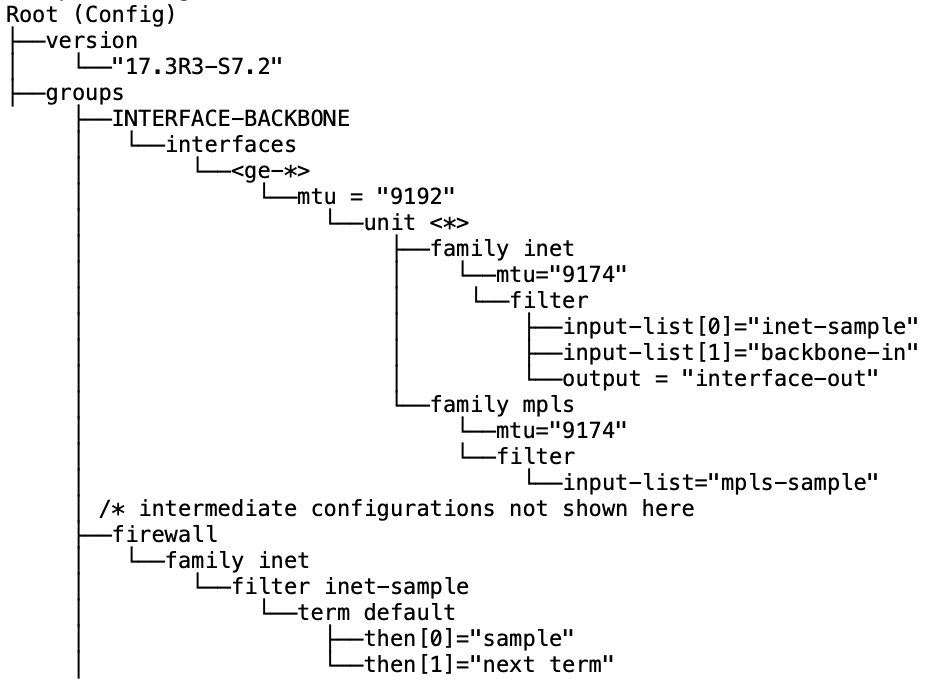
\includegraphics[width=0.85\columnwidth]{figs/tree_form.png}}
    \caption{Example snippet of tree-formatted Junpiter router configuration file.}
    \label{fig:tree}
\end{figure}

    \mypara{2. Contextual Relevance from Different Aspects} We make the observation that the context related to any given configuration line can be categorized into three types based on its position and relation within the configuration file as shown in the example in Figure~\ref{fig:context_mine}, with increasing levels of complexity to mine. They each providing unique insights that contribute to accurate misconfiguration detection: 
    
    \mysubpara{Neighboring Configurations} are those that are closely related to the line under examination, typically within the same section or functional block of the network configuration. For instance, if analyzing a line that defines a VLAN assignment on a particular interface, neighboring configurations would include other lines that configure the same interface or VLAN. These configurations provide insights into how related parameters are set up in proximity, revealing potential dependencies or conflicts. Additionally, by referencing related configurations that define or modify these neighboring parameters, one can understand how changes in one part of the network might impact adjacent configurations, helping to identify misconfigurations that could lead to issues like traffic misrouting or security vulnerabilities. Neighboring configurations are relatively easy to mine because they are identified based on adjacency or location in the configuration file, making them straightforward to extract.
        
    \mysubpara{Similar Configurations} involve the same type of parameter or function as the configuration line under review but are applied in different contexts within the network. For example, consider configurations that assign IP addresses to different interfaces across various routers in the network. Even though the interfaces and routers may differ, the principles governing IP address assignment remain the same. By comparing these similar configurations, one can detect inconsistencies or deviations from standard practices that might indicate a misconfiguration. This type of context is essential for ensuring that configuration practices are consistent across the network, reducing the risk of errors that could lead to network outages or performance degradation. Mining these configurations is more challenging because, unlike neighboring configurations, they are not located adjacently but must be identified based on functional similarities.

    \mysubpara{Referenceable Configurations}
    provide essential definitions or additional information related to the parameter value being examined. In the network domain, this context is crucial for understanding how specific values are applied across different parts of the network configuration. For example, if a parameter value specifies an import policy, referenceable configurations might include other lines where this policy is defined or where its behavior is modified. By examining these configurations, one can gain a deeper understanding of how the policy influences routing decisions or interacts with other network elements, ensuring that the configuration is applied correctly and consistently throughout the network.
    Referenceable configurations are the most difficult to mine because they often involve indirect references and dependencies that are not immediately apparent, requiring a thorough and sometimes recursive analysis to trace how a value or policy is used across various parts of the configuration file.

\begin{figure}[t]
    \centering
    \fbox{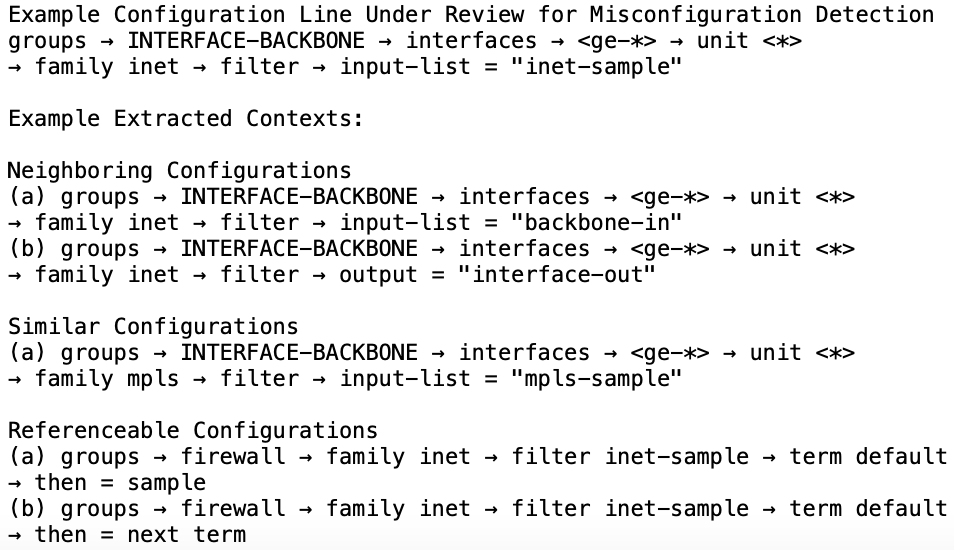
\includegraphics[width=0.85\columnwidth]{figs/context_mine.png}}
    \caption{Example context mined on selected config line.}
    \label{fig:context_mine}
\end{figure}

Given the categorization of relevant contexts and the hierarchical tree model, we can automate the process of mining the aforementioned contexts by translating them into specific paths within the tree. This involves the following steps:

\paragraph{Neighboring Configuration Mining:}
    Following the hierarchical tree structure of the configuration file, we can model the entire configuration as a tree \( T \) with nodes representing configuration elements and edges depicting the relationships between them. The root node \(V_1\) represents the entry point of the configuration file and the \(V_2\) nodes represent the broadest configuration categories.
    For a given configuration path \( P = \{ V_1 \rightarrow V_2(P) \rightarrow V_3(P) \rightarrow \dots \rightarrow V_k(P) = v_k(P) \} \) within the tree, where \( v_k(P) \) is the parameter value assigned to the parameter node \( V_k(P) \), the goal of neighboring configuration mining is to extract other paths in the tree that share a common sub-path with \( P \) up to a certain depth. 
    
    The common ancestry level, or shared node depth, can be adjusted to control how much context is mined. Let us define \( m \) as the number of shared nodes from the root, then neighboring configurations are defined as:
\begin{multline*}
N_m(P) = \{ P' \in T \mid P' = V_0 \rightarrow  V_1(P')\dots \rightarrow V_m(P') \rightarrow \\ V_{m+1}(P') \rightarrow \dots \rightarrow V_k(P')= v_k(P') \},
\end{multline*}

where \( P' \) shares the first \( m \) nodes with \( P \), but the nodes following \( V_m(P') \) (denoted as \( V_{m+1}(P'), V_{m+2}(P'), \dots \)) can differ from the remaining nodes in \( P \), and 
\(P'\) does not end at the same parameter node as \(P\), \ie, \( V_k(P') \neq V_k(P) \).




Adjusting \( m \) allows for control over the size and relevance of the neighboring context.
A common choice is to set \(V_m(P) = V_m(P') = V_{k-1}(P) \), which captures sufficient context while avoiding unnecessary complexity. For example. let the configuration path under review be represented as
\[
P = \{V_0 \rightarrow A \rightarrow B \rightarrow C \rightarrow D = v_D \} \mid V_{k-1}(P) = C
\]
The set of neighboring paths \( N(P) \) can be defined as:
\[
N(P) = \{ P' \in T \mid P' = V_0 \rightarrow A \rightarrow B \rightarrow C \rightarrow D' = v_{D'}, D' \neq D \}
\]
For example, consider a configuration line that defines the IP address for a particular interface:
\begin{multline*}
P = \{V_1 \rightarrow \text{interfaces} \rightarrow \text{ge-0/0/0} 
\rightarrow \text{unit 0} \rightarrow \text{family inet}\\
\rightarrow \text{address} = 192.168.1.1/24 \}
\end{multline*}
Here, \(V_{k-1}(P)\) would be \( \text{`family inet'} \). Neighboring paths in this case might include:
\begin{multline*}
N(P) = \{V_1 \rightarrow \text{interfaces} \rightarrow \text{ge-0/0/0}
\rightarrow \text{unit 0} \rightarrow
\text{family}\\ \text{inet} \rightarrow \text{mtu} = 1500 \}
\end{multline*}
This ensures the extracted neighboring paths are closely relevant, revealing how related parameters are configured in the same section without overwhelming the system with excessive data. Thus, in our evaluation of \sysname{}, we select \(V_{k-1}(P)\) as  \( V_m(P) \) for an effective balance between relevance and computational efficiency.


% \paragraph{Similar Configuration Mining:} To identify similar configurations, we locate paths that share the same entry point root node, the broadest category node (\(V_1\) and \(V_2\)), and parameter node (\(V_k\)) but vary in their intermediate nodes or parameter values. Let us again have \( P = \{ V_1 \rightarrow V_2(P) \rightarrow V_3(P) \rightarrow \dots \rightarrow V_k(P) = v_k(P) \} \) to represent a configuration line under review.
% Given \( P \), the set of similar configuration paths \( S(P) \) can be defined as:
% \begin{multline*}
% S(P) = \{ P' : P' = \{ V_1 \rightarrow V_2(P') \rightarrow V_3(P') \rightarrow \dots \rightarrow V_k(P') \\= v_k((P')) \} \},
% \end{multline*}
% where \( P' \) has \(V_2(P') = V_2(P)\) and \(V_k(P') = V_k(P)\), but can have any number of intermediate nodes (\( V_3(P'), V_4(P'), \dots \)) that differ from the intermediate nodes in \( P \), as well as possibly differing parameter value \( v_k(P') \) that does not equal to \( v_k(P) \).
% % The reason we use the \( L_1 \) node \( A \) rather than the root node \( V_0 \) is that the \( L_1 \) node represents the broad configuration category or section under which the parameter node \( D \) exists. 
% We make sure that any path \(P'\) in \(S(P)\) has \(V_2(P') = V_2(P)\) to 
% % By focusing on the same \( L_1 \) node, we 
% ensure that we are comparing similar types of configurations within the same category or context, even though the specific paths leading to \( V_k(P') \) and  \( V_k(P) \) may vary. Using only identical root node \( V_1 \) would not provide meaningful differentiation, as it encompasses the entire configuration file, making it too general for this analysis. By comparing these variations, we can understand how the same type of parameter is configured, which is essential for ensuring consistency across the network configuration.

\paragraph{Similar Configuration Mining:} To identify similar configurations, we focus on paths that share the same root node (\(V_1\)), broadest category node (\(V_2\)), and parameter node (\(V_k\)), but differ in their intermediate nodes or parameter values. Let \( P = \{ V_1 \rightarrow V_2(P) \rightarrow V_3(P) \rightarrow \dots \rightarrow V_k(P) = v_k(P) \} \) represent the configuration line under review again.
The set of similar configuration paths \( S(P) \) is defined as:
\begin{multline*}
S(P) = \{ P' : P' = \{ V_1 \rightarrow V_2(P') \rightarrow \dots \rightarrow V_k(P') = v_k(P') \} \},
\end{multline*}
where \( P' \) shares \(V_2(P') = V_2(P)\) and \(V_k(P') = V_k(P)\), but may have different intermediate nodes (\( V_3(P'), V_4(P'), \dots \)) and a different parameter value \( v_k(P') \).

By ensuring \(V_2(P') = V_2(P)\), we compare configurations within the same category or context, even if the paths leading to \( V_k(P') \) and \( V_k(P) \) differ. Using only the root node \( V_1 \) would be too broad, as it encompasses the entire configuration file and does not provide meaningful differentiation. This approach allows us to understand how the same type of parameter is configured across different instances, which is crucial for ensuring consistency in network configurations.



For example, let the configuration path under review be:
\[
P = \{ V_1 \rightarrow \text{Interfaces} \rightarrow \text{Ethernet0} \rightarrow \text{IP} \rightarrow \text{MTU} = 1500 \}
\]
This represents the configuration for setting the Maximum Transmission Unit (MTU) to 1500 on interface Ethernet0.
A similar configuration \( P' \) could be:
\[
P' = \{ V_1 \rightarrow \text{Interfaces} \rightarrow \text{Ethernet1} \rightarrow \text{IP} \rightarrow \text{MTU} = 9000 \}
\]
In this case, \( P' \) shares the same broad configuration category `Interfaces' (\( V_2(P') = V_2(P) \)) and parameter node `MTU' (\( V_k(P') = V_k(P) \)), but differs in the intermediate node `Ethernet1' and the parameter value (9000 vs. 1500). By comparing similar configurations, the context reveals not only the MTU settings but also the intermediate configuration elements leading to the MTU setting across different interfaces within the network configuration.


\paragraph{Referenceable Configuration Mining:} In the hierarchical tree structure, referenceable configurations are identified by locating paths where the parameter node of the current line under review appears as an intermediate node in other paths. This context is crucial for understanding how specific parameter values or policies are further referenced, elaborated upon, or applied in other parts of the configuration. we can formalize this set of referenceable configuration paths as:
\[
R(P) = \{ P' : P' =  V_1 \rightarrow \dots \rightarrow v_k(P) \rightarrow \dots \rightarrow V_k(P') \} = v_k(P').
\]
In these paths, \( v_k(P) \) is no longer a parameter value, but an intermediate node, meaning it is being referenced or defined further down the configuration hierarchy.

For example, suppose the current configuration line is:
\(V_1 \rightarrow RouterA \rightarrow Policy \rightarrow ImportPolicy = PolicyX\), a referenceable path might be:
\(
V_1 \rightarrow  RouterA \rightarrow Policy \rightarrow PolicyX \rightarrow Filter = AllowAll
\),
indicating that \( PolicyX \) is further applied or modified by the filter configuration. Referenceable configuration mining helps to understand not only how a particular configuration value is defined, but also how it interacts with or influences other components of the network. This process is essential for detecting misconfigurations that arise from improper application or dependency handling across different sections of the configuration file.


% By structuring the context mining process in this manner, we can efficiently and accurately extract the most relevant information for any given configuration line, enhancing the performance and accuracy of LLM-based configuration verification tools. This approach ensures that the LLM receives a well-curated set of contextually relevant data, improving its ability to detect sophisticated misconfigurations that depend on a comprehensive understanding of the configuration file.

However, one of the key problems in extracting referenceable configurations is the risk of pulling in irrelevant context, particularly because the process doesn't differentiate between pre-defined parameter values inherent to the configuration language and custom values defined by network administrators. 
% This lack of distinction can lead to incorrect or unnecessary context being extracted, as the system may treat a built-in parameter value the same as a user-defined one, resulting in inaccurate or misleading insights. 
We now proceed to discuss this problem in more detail and present our solution.

\subsubsection{Challenge 2 - Referenceable Parameter Value Ambiguity}

In network configurations, parameter values can broadly be categorized into two types: \textit{pre-defined} values and \textit{user-defined} values. Pre-defined values are those that are built into the configuration language itself, such as boolean flags (True vs. False) or access control decisions (Allow vs. Deny). These values are universally understood by the configuration parser and typically do not require any additional definition or context within the configuration file. On the other hand, user-defined values are customizable by the network administrator and can vary widely depending on the specific requirements of the network. These include values such as IP addresses, timeout intervals, VLAN IDs, and other numeric or alphanumeric identifiers. However, there rarely exists documentation explicit specifying these types and requires a lot of manual examination, which is hard to scale.

When extracting context for referenceable configurations,
failing to differentiate between pre-defined and user-defined values can introduce irrelevant or misleading information into the extracted context.
For instance, a pre-defined value like True is universally recognized by the configuration parser and could be used in multiple contexts, such as enabling a feature (FeatureX → Enabled = True) or setting a protocol flag (OSPF → PassiveInterface = True). Mining based on this pre-defined value could lead to irrelevant results, pulling in unrelated configurations that share the same boolean logic, thereby contaminating the context pool.
Conversely, user-defined values like IP addresses, a prefix limit (\eg, "maximum-prefixes 500" in a BGP configuration) or a timeout interval (\eg, 30 seconds) are specific to the network and typically set by network operators. These values may appear in routing tables, NAT rules, or timeout policies, with their significance depending on how they’re defined and applied. In this case, mining should focus on retrieving all related configurations that define or use these values.

Distinguishing between pre-defined and user-defined values is crucial to avoid extracting irrelevant context, which can lead to several issues:


\begin{enumerate}
    \item \textit{Context Contamination}: 
    Irrelevant context introduced during the context mining process might erroneously group together configurations that pertain to entirely different aspects of network operation.
    % thereby confusing the LLM and reducing the accuracy of its inferences.
    This contamination of the context pool dilutes the relevance of the mined information, reducing the precision of the LLM and increasing the likelihood of false positives or missed errors. 
    \item \textit{Reducing Computational Costs}: LLMs can be computationally expensive, especially when processing large-scale network configurations with many interdependent components. Distinguishing between pre and user-defined values can help optimizing the context extraction process, ensuring that only relevant and necessary contexts are passed to the model. This reduces the computational overhead associated with processing extraneous information.
    % For instance, consider the case of mining context for a user-defined IP address. Suppose a configuration line specifies Interface → IPAddress = 192.168.1.1. In this case, the relevant context might include other configurations that reference this specific IP address, such as firewall rules or routing entries. However, if the mining process mistakenly treats Allow or True in the same way as user-defined values, it might pull in unrelated contexts from access control lists or feature flags, resulting in unnecessary processing and potentially higher costs.

\end{enumerate}

\mypara{Existence and Majority-Voting Based Differentiation}
To accurately differentiate between pre-defined and user-defined parameter values within configuration files, we propose a solution that combines existence checks within the configuration tree and a majority-voting mechanism.

\mysubpara{1. Existence-Based Differentiation:}
User-defined values often carry contextual information and are typically associated with further definitions or explanations elsewhere in the configuration file. For example, if a parameter value represents a specific, customized import policy, the configuration should contain other lines that elaborate on this policy's behavior. In the hierarchical tree model, if a parameter value is user-defined, it is likely to appear as an intermediate node in other configuration paths, indicating that it is referenced or elaborated upon elsewhere. Conversely, if no such paths exist, the value is likely pre-defined and requires no additional context. Consider the parameter RoutingPolicy with a value of ImportPolicy1 as an example. If ImportPolicy1 appears as an intermediate node in other configuration lines, such as those defining specific route maps or filters, it is likely user-defined. On the other hand, a parameter value like `PassiveInterface = True' might not have any additional references, indicating that True is a pre-defined value.

Formal Definitions:
Let \( \text{Val}_{\text{user}} \) be the set of user-defined values, and \( \text{Val}_{\text{pre}} \) be the set of pre-defined values.
A parameter value \( v_k \) is considered \textit{user-defined} if it appears as an intermediate node in at least one other configuration path \( P' \in T \). This can be expressed as:
\begin{multline*}
v_k \in \text{Val}_{\text{user}} \iff \exists P' = \{ V_1 \rightarrow \dots \rightarrow v_k \dots \rightarrow V_k(P') \\ = v_k(P') \} \in T
\end{multline*}

A parameter value \( v_k \) is considered \textit{pre-defined} if it does not appear as an intermediate node in any other configuration path \( P' \in T \). This can be formalized as:
\begin{multline*}
v_k \in \text{Val}_{\text{pre}} \iff \nexists P' = \{ V_1 \rightarrow \dots \rightarrow v_k \dots \rightarrow V_k(P') \\ = v_k(P') \} \in T
\end{multline*}


% There are edge cases where this approach is less applicable. Some parameter values, such as numeric ranges or flexible inputs, may not have explicit definitions within the configuration. However, these are generally treated as pre-defined since they are standardized and do not require further explanation.


\mysubpara{2. Majority-Voting for Consistency:} A shortcoming with existence-based differentiation is that the same parameter value can be user-defined in one context and pre-defined in another. For instance, the value 1000 used in a timeout setting might be pre-defined and require no further explanation. However, the same value 1000 used as a policy name or group identifier could be user-defined and require contextual elaboration. This distinction is crucial, as identical values can have different meanings depending on the associated configuration parameter. To address this ambiguity, we avoid assigning a universal type to a parameter value across all configurations. Instead, we determine whether a value is pre-defined or user-defined based on the specific combination of the configuration parameter and its associated value. For each configuration parameter, we analyze all associated values. If the majority of these values are user-defined, we classify the entire parameter (\(V_k\)) as well as all of its possible values (\(v_k\)) as user-defined. Conversely, if the majority are pre-defined, the parameter is classified accordingly. This approach leverages the principle that configuration parameters should exhibit uniformity in the type of values they accept, maintaining consistency across the configuration.

This further transforms our previous definition of \( \text{Val}_{\text{user}} \)  and \( \text{Val}_{\text{pre}} \)  into:
\[
(V_k, v_k) = 
\begin{cases} 
\text{User-Defined}, \text{if } \sum_{i=1}^{n} \mathbb{1}(v_i \in \text{Val}_{\text{user}}) > \frac{n}{2}, \\
\text{Pre-Defined}, \text{if } \sum_{i=1}^{n} \mathbb{1}(v_i \in \text{Val}_{\text{pre}}) \geq \frac{n}{2}.
\end{cases}
\]
where \( n \) is the number of unique values associated with the configuration parameter \( V_k \), and \( \mathbb{1} \) is the indicator function that checks whether a value is user-defined or pre-defined.


Example: For the parameter Timeout, where values like 1000, 2000, and 3000 are used, if the majority lack associated definitions, they are treated as pre-defined. Conversely, for a parameter like ImportPolicy, where values such as PolicyA, PolicyB, and 1000 (as a policy name) are used, if most have contextual definitions, all values under that parameter are treated as user-defined.


By combining existence-based checks with a majority-voting mechanism, we can effectively differentiate between pre-defined and user-defined parameter values in network configurations. This method ensures that the context extracted for LLM analysis is both relevant and accurate, thereby enhancing performance and reducing computational costs. Moreover, this approach maintains consistency within the configuration, ensuring that similar parameters are uniformly treated across different contexts.


\subsection{Iterative Prompting}\label{prompting_method}
As we transition from context mining to utilizing the extracted information in LLM prompts, the next challenge is how to feed this information into the model without overwhelming it. While extracting accurate and relevant context is essential, the model's ability to process that information effectively is just as crucial.

% A significant limitation of many LLM-based approaches is context overload, where the model is fed too much information at once, causing it to lose focus on the most pertinent details. This is especially relevant in network configurations, where dependencies and relationships between different configuration lines can be complex and spread throughout the file.

\subsubsection{Challenge 3 - Context Overload in Prompting}
\label{challenge_3}
A significant limitation of many LLM-based approaches is context overload, where the model is fed too much information, causing it to lose focus on the most pertinent details. This is especially relevant in network configurations, where dependencies and relationships between different configuration lines can be complex and spread throughout the file.
Even with the precise context extraction mechanisms we have, the extracted context can sometimes be extensive. 
% When this large amount of context is provided to an LLM in a single prompt, the model can struggle to maintain focus, leading to several issues:
Feeding this large amount of context to an LLM can lead to several issues:
\begin{enumerate}
    \item \textit{Dilution of Relevance}: The model might lose track of the most critical elements of the prompt, resulting in responses that are less accurate or less relevant. For instance, in a complex router configuration, key misconfiguration details could get buried in a flood of less relevant context.
    \item \textit{Loss of Coherence and Accuracy}: The model might generate responses that are disjointed or fail to address the core misconfiguration, as it attempts to process all the given information at once. This can lead to fragmented reasoning or erroneous conclusions when handling intricate dependencies in router settings. Additionally, LLMs have inherent token limitations, and overloading the prompt with context can force the model to either truncate important sections or attempt to process more than it reasonably can, which can also severely impact performance.
    % \item \textit{Decreased Performance}: Providing too much context can overwhelm the model’s processing capabilities, degrading the overall quality of the output. LLMs have inherent token limitations, and overloading the prompt with context can force the model to either truncate important sections or attempt to process more than it reasonably can, which can severely impact performance.
\end{enumerate}

For example, in detecting routing policy misconfigurations, a single misconfigured line may have dependencies across several sections of the file. Presenting all related context at once can cause the model to fail at prioritizing critical information, leading to missed/incorrect detection. STOA methods, such as prompt chaining, which guides the model through chained instructions, doesn't solve this issue, as it doesn't dynamically adjust or prioritize the context based on model needs.


\mypara{Solution}
To combat these issues, \sysname{} implements an iterative, sequential prompting framework that allows the model to request and process relevant context in stages. Instead of overwhelming the model with all available context at once, \sysname{} enables the model to actively request additional information as needed. This approach enhances the model’s ability to maintain focus, coherence, and overall detection accuracy by allowing it to prioritize and process context more effectively, ensuring that only the most pertinent information is presented at each step.

\mysubpara{1. Initial Prompting:} The process begins by feeding the LLM the specific configuration line under review, along with targeted instructions about the type of misconfiguration we are checking for (\eg, syntax errors, dependency conflicts, or just general misconfiguration). This prompt is concise, providing only the critical line and the request as shown in the Figure~\ref{fig:initial_prompt}. This reduces the initial information load and allows the model to focus on the core issue.


    \begin{figure}[tb]
    \centering
    \fbox{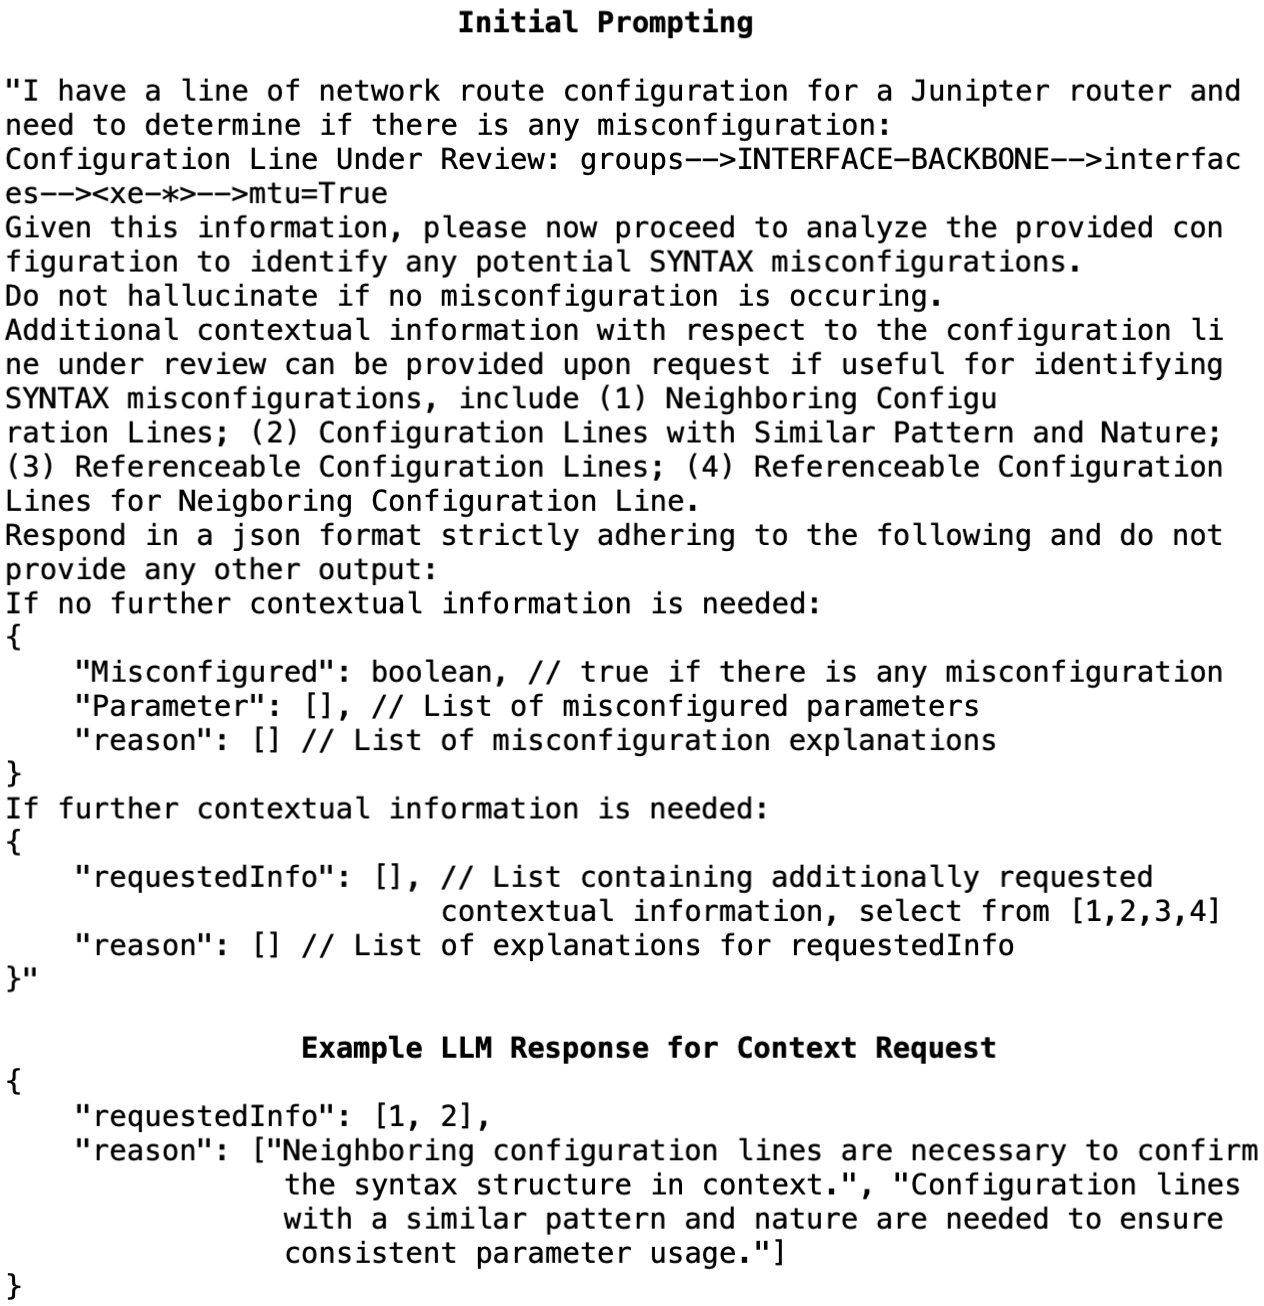
\includegraphics[width=\columnwidth]{figs/initial_prompt_response.png}}
    \caption{Example: initial prompting and LLM context request response for detecting syntax misconfiguration.}
    \label{fig:initial_prompt}
\end{figure}

\mysubpara{2. Contextual Options:} Next, \sysname{} offers the model the option to request additional context based on its understanding of the configuration line and the misconfiguration detection request. These options are based on our categorized context types, including: neighboring (\( N(P) \)), similar (\(S(P) \)) , and referenceable contexts (\( R(P) \)), as well as referenceable contexts on neighboring configurations (\( N(R(P)) \)). By allowing the model to choose which context to receive, \sysname{} ensures that the LLM is only given information that is most relevant to the detection task at hand, reducing the risk of context overload. An example request response is shown in Figure~\ref{fig:initial_prompt}.
    
\mysubpara{3. Iterative Refinement:} After the model processes the initial prompt, it can request additional information if needed before arriving at the final decision. \sysname{} engages in a feedback loop where the model’s output informs the next set of prompts. For instance, if the model identifies a possible syntax issue but requires more context from a related policy definition, \ie, similar context, \sysname{} can deliver that specific context in the next prompt. This iterative process continues until the model has sufficient information to make a well-informed decision. Figure~\ref{fig:feedback_and_response} provides an example of what a final misconfiguration decision looks like.
    \begin{figure}[tb]
    \centering
    \fbox{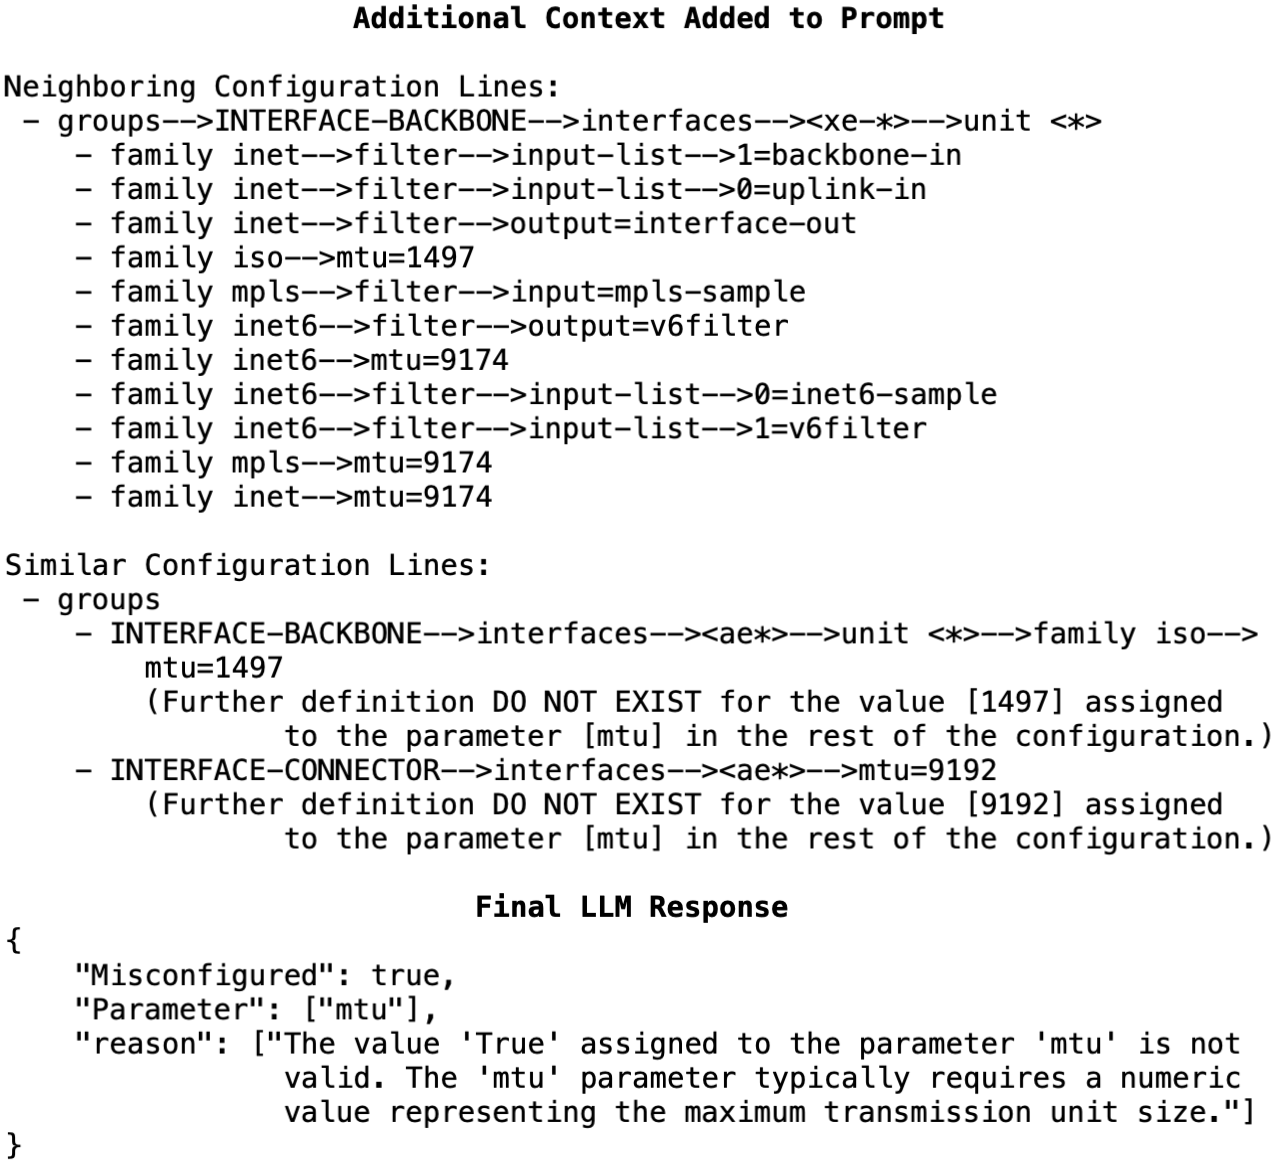
\includegraphics[width=\columnwidth]{figs/feedback_and_response.png}}
    \caption{Example: Adding requested context and retrieving misconfiguration detection result.}
    \label{fig:feedback_and_response}
\end{figure}


This sequential, interactive approach mirrors how a network administrator might manually review a configuration file—examining the most relevant sections first, then digging deeper into referenceable or adjacent configurations as needed. It ensures that the model focuses on the most critical aspects of the configuration without becoming overwhelmed by extraneous information.

\subsubsection{Why Iterative, Requested Based Prompting Works}
By breaking down the context into smaller, more digestible portions, \sysname{} addresses the fundamental challenges of context overload. This method significantly enhances the model’s ability to:
\begin{enumerate}
    \item Stay on target: With less irrelevant information, the model can maintain focus on the specific issue under review.
    \item Preserve coherence: Incrementally adding information allows the model to build a more coherent understanding of the configuration~\cite{li2023prompt,subramonyam2024bridging}, improving detection of complex issues such as dependency conflicts or misapplied policies.
    \item Optimize performance: Avoiding context overload reduces the processing burden on the model, leading to faster and more reliable outputs.
\end{enumerate}

For example, in detecting misconfigurations in a multi-layer firewall policy, \sysname{} might first present the core rule in question, then iteratively offer neighboring rules that affect the same traffic flow, followed by referenceable configuration sections that define broader network policies. This structured process ensures that the LLM has all the information it needs, without drowning in unnecessary details, enabling it to make accurate decisions. Unlike conventional prompt-chaining, which provides incremental instructions based on a fixed context, \sysname{} dynamically adds context as requested by the LLM, focusing on the evolving needs of the analysis.

% By combining efficient context extraction with iterative, focused interaction, \sysname{} represents a significant advancement in leveraging LLMs for router misconfiguration detection, ensuring that models are both effective and computationally efficient.
\section{Evaluation}
\label{sec:eval}
To evaluate the effectiveness of \sysname{}, we present three test scenarios as case studies and compare \sysname{} with state-of-the-art solutions. These include:
\begin{enumerate}
    \item A comprehensive set of common misconfiguration types, where synthetic misconfigurations representing these types are introduced into collected network configurations.
    \item A set of real-world misconfigurations verified in actual network configurations.
    \item An exhaustive run of \sysname{} on the entire configuration file of a medium-scale campus network to assess its ability to identify new misconfigurations.
    
We now introduce the setup for our evaluation.
\end{enumerate}
\subsection{Evaluation Setup}
\subsubsection{Context Extraction Hardware Setup}


\textit{System Information}: GNU/Linux Red Hat Enterprise Linux release 8.8 (Ootpa);

\textit{CPU Specifications}: Architecture: x86\_64; CPU(s): 32 (2 threads/core, 16 cores/socket, 1 socket); Model: AMD EPYC 7302P 16-Core Processor; Max MHz: 3000.000; L3 cache: 16384K; NUMA node0 CPU(s): 0-31 

We opt not to use the GPU, as the computational cost of the context extraction and processing tasks was manageable on the CPU. The detailed resource profiling shows that the tasks primarily benefit from parallel CPU threads, and GPU acceleration would not provide significant additional speedup.


\subsubsection{LLM Model Used: GPT-4o} For running the LLM-based detection, we use GPT-4o, OpenAI's most advanced transformer-based model designed for complex multi-step tasks.
\textit{Model Specifications}:
\begin{itemize}
    \item Model: GPT-4o-2024-05-13
    \item Context window: 128,000 tokens 
    \item Max output tokens: 4,096 tokens
    \item Training data Up to October 2023
\end{itemize}

\subsubsection{Prompting and Query Setup}
We use OpenAI’s Chat Completions API to interact with GPT-4o. The system was provided with a structured conversation history to maintain context across multiple queries. For each query, the model was tasked with analyzing the configuration file to detect potential misconfigurations, with instructions tailored to focus on specific misconfiguration types (e.g., syntax issues, policy conflicts) or general misconfigurations. Example prompting, queries, and responses are shown in Figures~\ref{fig:initial_prompt} and ~\ref{fig:feedback_and_response}.

\subsection{Case Study 1: Synthetic Misconfiguration Detection}
In this case study, we broadly categorize router misconfigurations into three types: (1) syntax errors, (2) range violations, and (3) dependency/conflict issues.
\begin{itemize}
    \item \textit{Syntax errors} occur when the configuration syntax does not adhere to the expected format or structure. For example, a missing bracket or misused keyword in a BGP routing policy.
    \item \textit{Range violations} involve parameter values that fall outside the acceptable range. An example would be an MTU value that exceeds the maximum allowed for a specific interface type.
    \item \textit{Dependency/conflict} issues arise when different configuration lines are incompatible or contradict each other. For instance, a firewall rule might block traffic that another policy explicitly permits.
\end{itemize}

To evaluate \sysname{}, we first obtain snapshot configurations from Internet2 (Juniper devices) and introduce synthetic misconfigurations representing the three types. For each type, we create four distinct misconfigurations, resulting in a total of 12 misconfigurations. For each misconfiguration, we run \sysname{} by following the two components: (1) treating the misconfigured line as the line under review and extracting all relevant context, and (2) conducting the iterative, sequential prompting process against the model, obtaining the final misconfiguration detection decision.

When forming the prompt, we explicitly instruct the model to look for each type of misconfiguration—syntax, range, or dependency/conflict—individually. This is because the model may request different types of context depending on the specific misconfiguration type it is trying to detect. We report only the results corresponding to the actual misconfiguration type introduced. Importantly, \sysname{} never yielded false positives when the model was instructed to find a misconfiguration type different from the actual type. Additionally, we find that asking the model to search for `general' misconfigurations also led to successful detection, though more context was often requested by the model.

As a baseline, we compare \sysname{} to three representative tools: \textit{Batfish}, a model-checking tool, \textit{Diffy}, a data-mining-based tool, and a partition-based GPT Q\&A model using GPT-4o for fair comparison. We present the specific misconfigurations introduced and the results in Table X, demonstrating how each tool performed in detecting the synthetic misconfigurations across the three categories.

\subsection{Case Study 2: Real-World Misconfiguration Detection}
To reflect real-world misconfigurations, we obtain Juniper router configuration snapshots from a campus network where known misconfigurations regarding port assignment have been found using their graph-based verifier. We instruct the model to detect 'general' misconfigurations when prompting.

A key aspect of this case study is the demonstration of \sysname{}'s flexibility in integrating additional context types under different scenarios. For example, port assignment misconfigurations often require a network-wide view, as they often can only be accurately identified when the context of other devices within the same network is considered. To address this, we introduce an additional, default context type, called `Intra-Router Consistency Context.' This context type mines and evaluates the prevalence of the same parameter-value pair across other devices in the network, providing insights into whether a configuration is common or potentially erroneous.
Example Intra-Router Consistency Context extracted:

\textit{`For the Configuration Line Under Review, the same configuration is found in 189 out of 191 other configuration files. (Significantly lower prevalence may indicate an uncommon or potentially erroneous configuration.'}

We evaluate \sysname{}'s performance on these misconfigured lines and compare the results to the original graph-based verifier, \textit{Batfish}, and the partition-based GPT Q\&A model. The comparison of results is presented in Table X.

\subsection{Case Study 3: Large-Scale Network Misconfiguration Detection}
Lastly, we obtain Aruba router configuration snapshots from a medium-sized campus network. Unlike the previous scenarios, this dataset does not contain ground truth misconfigurations. The objective here is twofold: (1) to verify the scalability of \sysname{} when applied to larger network configurations, and (2) to investigate whether \sysname{} can detect potential misconfigurations that have not yet been identified by existing tools.

We perform an exhaustive analysis using \sysname{} across five full configuration files, applying the context mining framework to extract all relevant context for each configuration line. We then prompt the model to identify 'general' misconfigurations, allowing it to dynamically request the necessary context during the iterative prompting phase. The detection results are presented in Table X, highlighting \sysname{}'s ability to uncover new misconfigurations.
\section{Discussion and Future Work}
\label{sec:future}

\sysname{} has proven effective in improving the detection of router misconfigurations, but there are several avenues for further exploration and refinement. One notable challenge is expanding the framework to better handle large-scale, distributed networks with interdependent routers. These environments often involve complex relationships between devices, and future work could focus on extending \sysname{} to capture and analyze multi-device contexts by default. Incorporating cross-router consistency checks and advanced network-wide policy validation could be valuable enhancements.

Another area for improvement is enhancing the LLM's ability to process real-time configuration changes. As networks evolve dynamically, incorporating real-time monitoring data into the context mining process would allow for continuous verification and faster misconfiguration detection. Integrating \sysname{} with network management tools that track operational metrics could provide valuable runtime data, further improving detection accuracy by correlating live data with configuration snapshots.

Lastly, improving the interpretability and transparency of LLM decisions in \sysname{} is an area for future work. Providing clearer explanations for why certain misconfigurations are flagged could assist network operators in quickly understanding and addressing potential issues. Combining LLM-based reasoning with rule-based approaches might provide a more robust system that blends the strengths of both methodologies, offering accurate detection alongside actionable insights.
\section{Conclusion}
\label{sec:conclusion}

In this paper, we introduced \sysname{}, a framework for router misconfiguration detection that leverages context-aware iterative prompting to improve LLM accuracy. By systematically extracting relevant context from network configurations
and following a guided, interactive prompting mechanism, \sysname{} addresses limitations in current model checkers, consistency checkers, and LLM-based models. Through case studies involving both synthetic and real-world misconfigurations, we demonstrated that \sysname{} outperforms existing methods across different misconfiguration types, ensuring more reliable and scalable network configuration verification.
\label{endOfBody}
\bibliographystyle{plain}
\bibliography{citations} 
\end{sloppypar}
\label{LastPage}

\pagebreak
\end{document}